\documentclass[12pt]{article}
\usepackage[a4paper, total={6in, 9in}]{geometry}
\usepackage{graphicx}
\graphicspath{ {./images/output/} }
\usepackage{caption}
\usepackage[english]{babel}
\usepackage{titling}
\usepackage{float}
\usepackage{amsmath}
\usepackage{minted}
\usepackage{multicol}
% \usepackage{makecell}
\usepackage{tabularx}
\usepackage{multirow}
\usepackage{adjustbox}
% \usepackage{array}
% \usepackage{setspace}
% \usepackage{placeins}
\setlength{\parindent}{0pt}

% \usepackage{lipsum}

\title{Study of Digital Modulation (ASK, FSK, PSK)}
\author{}
\date{}

\pagenumbering{gobble}
\begin{document}
\vspace*{\fill}
\begin{center}

    \emph{Heaven's Light is Our Guide} \\
    \textbf{Rajshahi University of Engineering and Technology} \\

    \begin{figure}[H]
        \centering
        
\includegraphics[scale=.34]{images/RUET_logo.png}
        \label{fig:ruet_logo}
    \end{figure}
    \vspace{5mm}

    \textbf{Course Code}\\
    ECE 3208\\
    \vspace{3mm}
    \textbf{Course Title}\\
    Communication Engineering Sessional

    \vspace{5mm}
    \textbf{Experiment Date:} {January 21, 2025},\\
    \textbf{Submission Date:} {February 11, 2025}\\

    \vspace{5mm}
    \textbf{Lab Report 3: \\
        Determination of Modulation Index of FM Wave}

    \vspace{15mm}

    \begin{tabular}{c|c}
        \textbf{Submitted to} & \textbf{Submitted by} \\
        Dr. Md. Kamal Hosain  & Md. Tajim An Noor     \\
        Professor             & Roll: 2010025         \\
        Dept of ETE, RUET     &                       \\
    \end{tabular}

\end{center}
\vspace*{\fill}


\pagebreak

\tableofcontents

\pagebreak
\pagenumbering{arabic}
\maketitle

\section*{Theory}
\addcontentsline{toc}{section}{Theory}
Digital modulation transforms digital symbols into waveforms compatible with the transmission medium by varying the carrier signal's amplitude, frequency, or phase according to the digital data. The goal is to efficiently transmit data while maintaining signal integrity and minimizing errors. Common types include Amplitude Shift Keying (ASK), Frequency Shift Keying (FSK), and Phase Shift Keying (PSK) \cite{proakis2007digital}.

\subsection*{Amplitude Shift Keying (ASK)}
Amplitude Shift Keying (ASK) is a type of digital modulation where the amplitude of the carrier signal is varied in accordance with the binary data. The general form of an ASK signal is:
\[
    s(t) =
    \begin{cases}
        A \cos(2 \pi f_c t) & \text{if } m(t) = 1 \\
        0                   & \text{if } m(t) = 0
    \end{cases}
\]
where \( A \) is the amplitude, \( f_c \) is the carrier frequency, and \( m(t) \) is the message signal \cite{sklar2001digital}.

\subsection*{Frequency Shift Keying (FSK)}
Frequency Shift Keying (FSK) is a type of digital modulation where the frequency of the carrier signal is varied according to the binary data. The general form of an FSK signal is:
\[
    s(t) =
    \begin{cases}
        A \cos(2 \pi f_1 t) & \text{if } m(t) = 1 \\
        A \cos(2 \pi f_2 t) & \text{if } m(t) = 0
    \end{cases}
\]
where \( A \) is the amplitude, \( f_1 \) and \( f_2 \) are the frequencies for binary 1 and 0 respectively, and \( m(t) \) is the message signal \cite{haykin2001communication}.

\subsection*{Phase Shift Keying (PSK)}
Phase Shift Keying (PSK) is a type of digital modulation where the phase of the carrier signal is varied according to the binary data. The general form of a PSK signal is:
\[
    s(t) = A \cos(2 \pi f_c t + \theta)
\]
where \( A \) is the amplitude, \( f_c \) is the carrier frequency, and \( \theta \) is the phase shift. For Binary PSK (BPSK), the phase shift \( \theta \) is:
\[
    \theta =
    \begin{cases}
        0   & \text{if } m(t) = 1 \\
        \pi & \text{if } m(t) = 0
    \end{cases}
\]
where \( m(t) \) is the message signal \cite{lathi2009modern}.


\section*{Required Apparatus}
\addcontentsline{toc}{section}{Required Apparatus}
\begin{itemize}
    \item ETEK DCS-6000-06 (ASK Modulation \& Demodulation Kit)
    \item ETEK DCS-6000-07 (FSK Modulation \& Demodulation Kit)
    \item ETEK DCS-6000-08 (PSK(BPSK) Modulation \& Demodulation Kit)
    \item Oscilloscope
    \item Connecting Wires
    \item Power Supply
    \item Signal Generator (To make Square Waves to offset to mimic digital signal)
\end{itemize}

\section*{Diagrams}
\addcontentsline{toc}{section}{Diagrams}
\subsection*{Circuit Diagram of ASK System}
\begin{figure}[H]
    \centering
    % 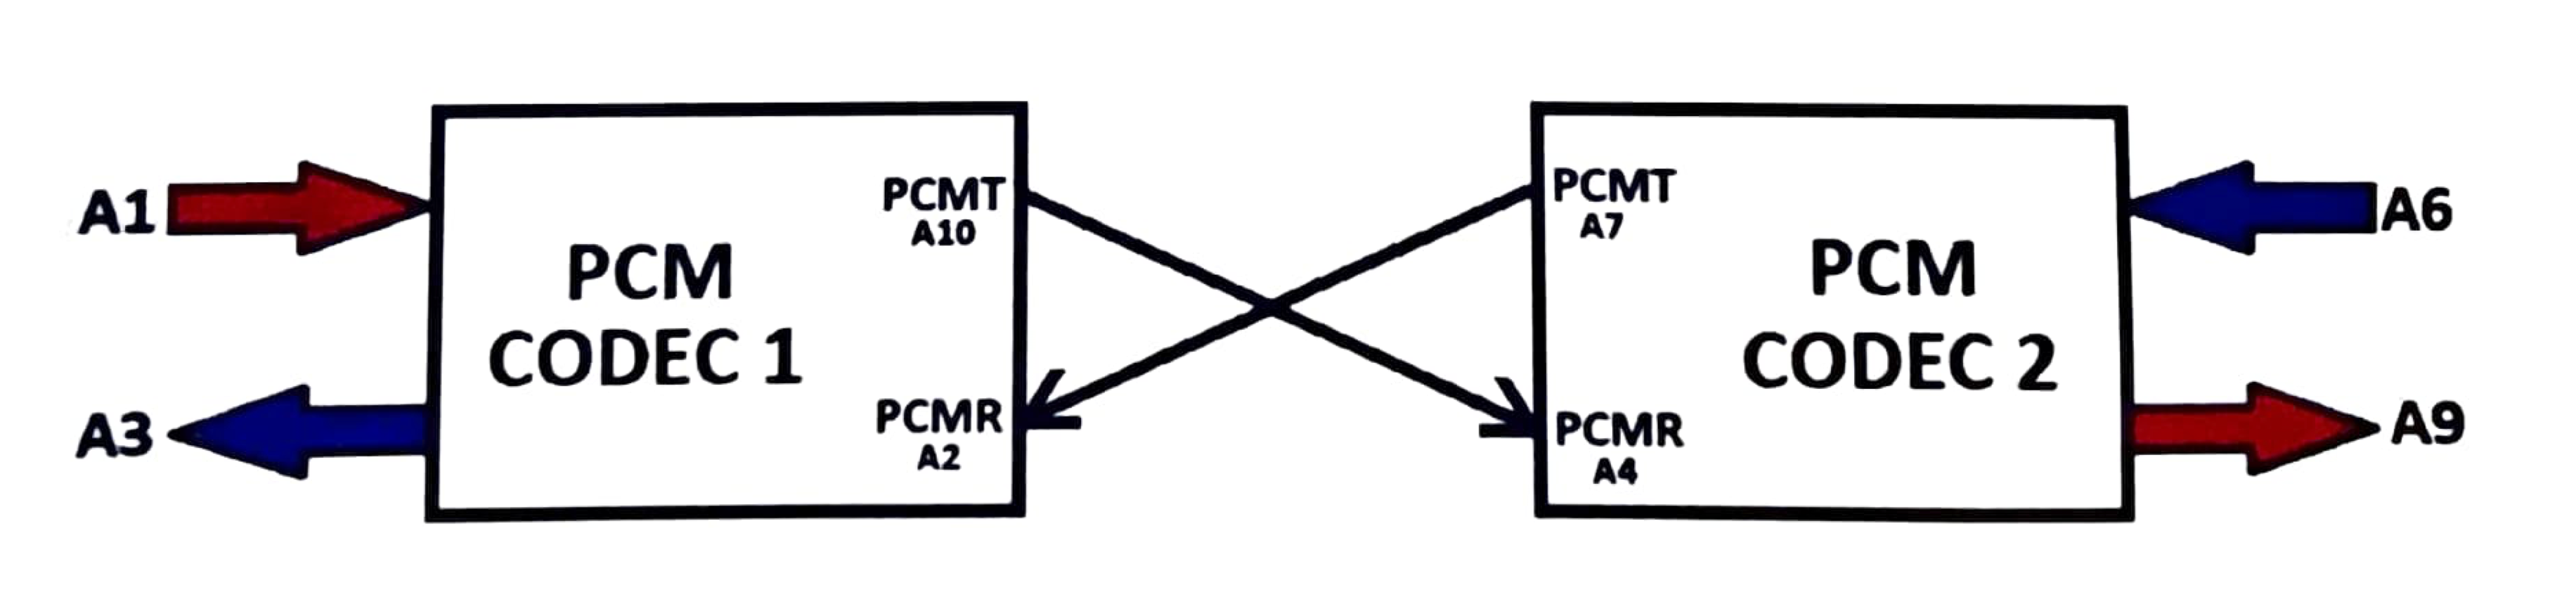
\includegraphics[width=.95\textwidth]{ckt.png}
    \caption{Circuit Diagram of ASK System}
    \label{fig:ask}
\end{figure}

\subsection*{Circuit Diagram of FSK System}
\begin{figure}[H]
    \centering
    % 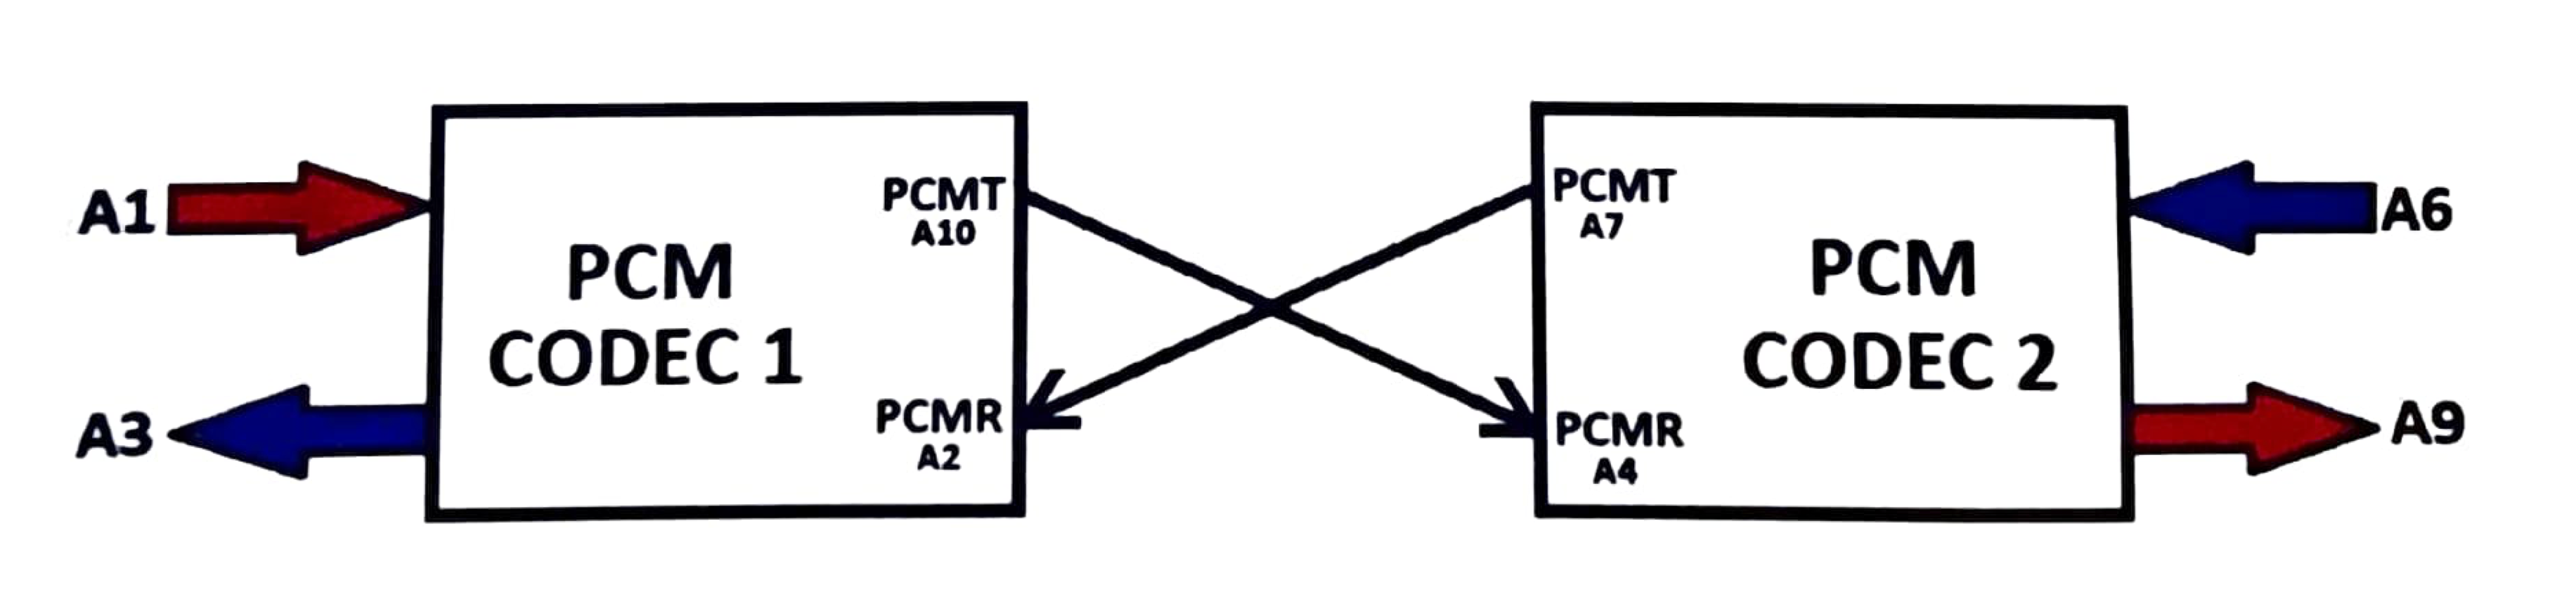
\includegraphics[width=.95\textwidth]{ckt.png}
    \caption{Circuit Diagram of FSK System}
    \label{fig:fsk}
\end{figure}

\subsection*{Circuit Diagram of PSK System}
\begin{figure}[H]
    \centering
    % 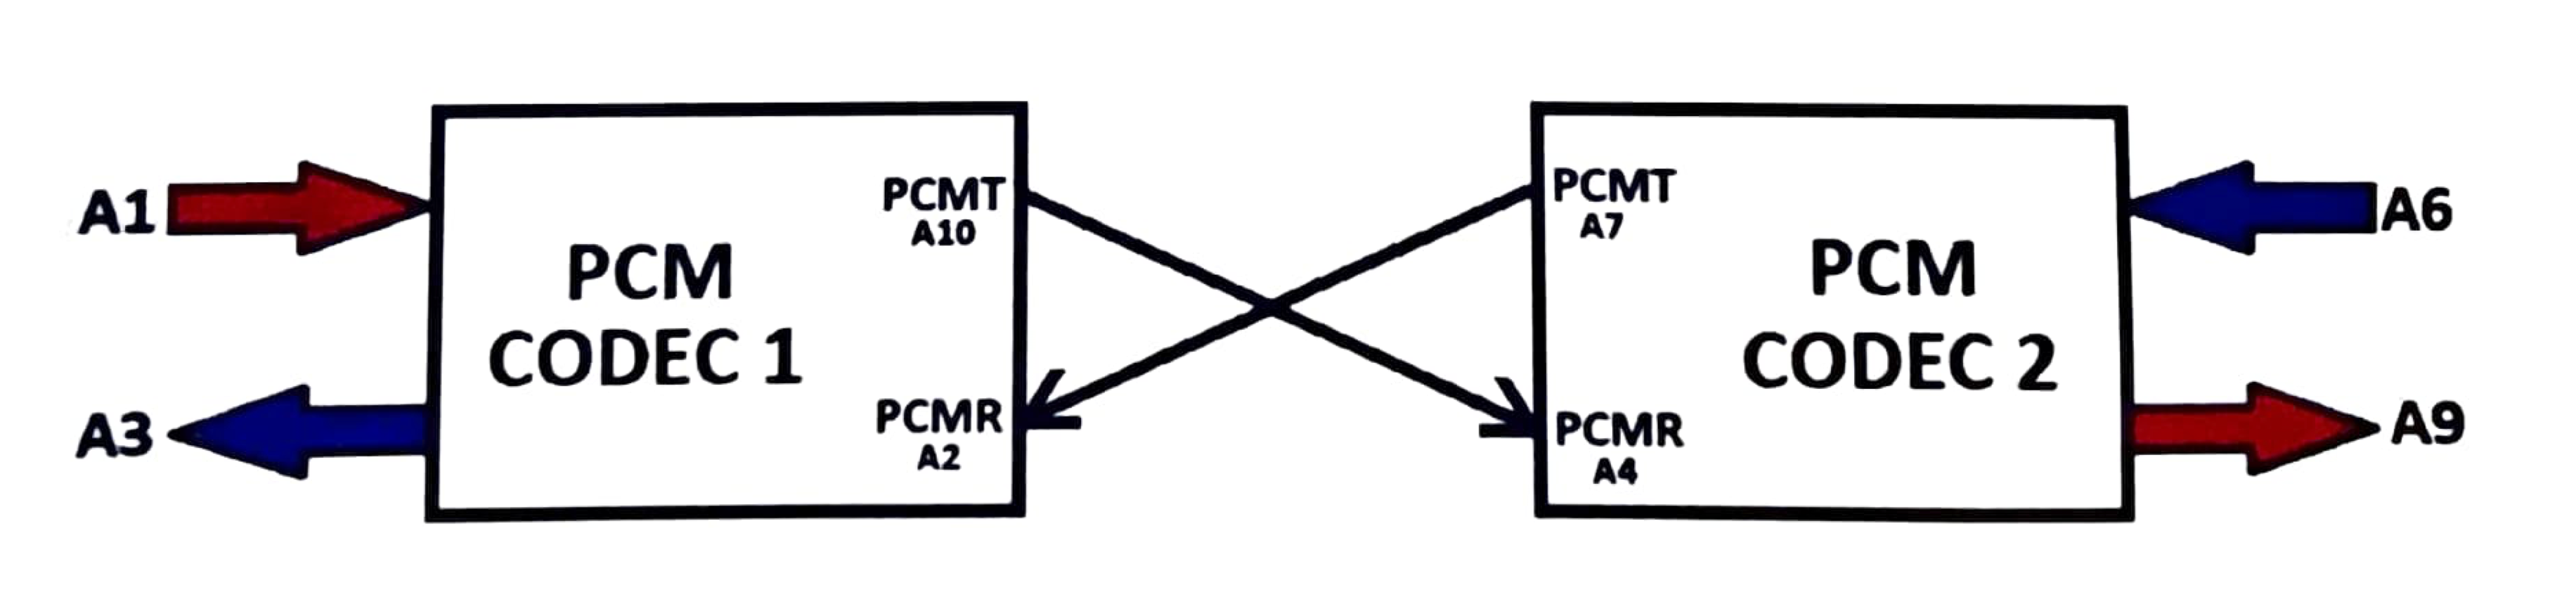
\includegraphics[width=.95\textwidth]{ckt.png}
    \caption{Circuit Diagram of PSK System}
    \label{fig:psk}
\end{figure}

\section*{Procedure}
\addcontentsline{toc}{section}{Procedure}
\begin{enumerate}
    \item The ASK Modulation \& Demodulation Kit (ETEK DCS-6000-06) was connected to the power supply.
    \item The signal generator was connected to the input of the ASK modulator to generate a square wave signal.
    \item The modulated ASK signal was observed on the oscilloscope.
    \item The output of the ASK modulator was connected to the input of the ASK demodulator.
    \item The demodulated signal was observed on the oscilloscope and compared with the original input signal.
    \item The above steps were repeated for the FSK Modulation \& Demodulation Kit (ETEK DCS-6000-07) and PSK(BPSK) Modulation \& Demodulation Kit (ETEK DCS-6000-08).
\end{enumerate}

% \section*{Experimental Data}
% \addcontentsline{toc}{section}{Experimental Data}

\section*{Observation}
\begin{itemize}
    \item In ASK, the amplitude of the carrier signal changes with the binary data: present for 1, absent for 0.
    \item In FSK, the frequency of the carrier signal changes with the binary data: \( f_1 \) for 1, \( f_2 \) for 0.
    \item In PSK, the phase of the carrier signal changes with the binary data: 0 for 1, \( \pi \) for 0.
    \item For ASK demodulation, the demodulated signal closely matches the original binary data by detecting the carrier signal's presence or absence, but it wasn't perfect.
\end{itemize}


\section*{Matlab Simulation}
\addcontentsline{toc}{section}{Matlab Simulation}

\subsection*{Code:}
\addcontentsline{toc}{subsection}{Code}
\inputminted[linenos,breaklines,breakanywhere]{matlab}{./assets/dsk.m}

\section*{Output}
\addcontentsline{toc}{section}{Output}

\subsection*{Experimental Output}
\addcontentsline{toc}{subsection}{Experimental Output}
\begin{figure}[H]
    \centering
    \begin{minipage}{0.45\linewidth}
        \centering
        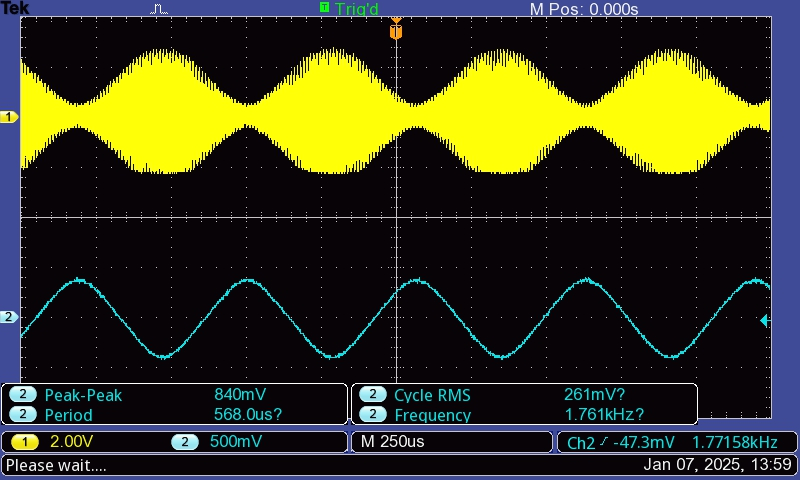
\includegraphics[width=\linewidth]{p1-undMod-msg.JPG}
        \caption{AM; Yellow: Under-modulated, Blue: Message}
        \label{fig:pic1}
    \end{minipage}
    \hfill
    \begin{minipage}{0.45\linewidth}
        \centering
        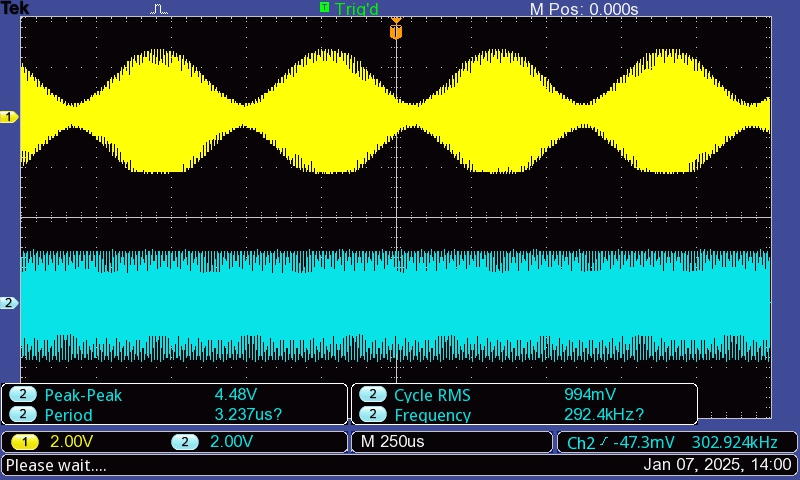
\includegraphics[width=\linewidth]{p2-undMod-car.JPG}
        \caption{AM; Yellow: Under-modulated, Blue: Carrier}
        \label{fig:pic2}
    \end{minipage}
    \vspace{1em}
    \begin{minipage}{0.45\linewidth}
        \centering
        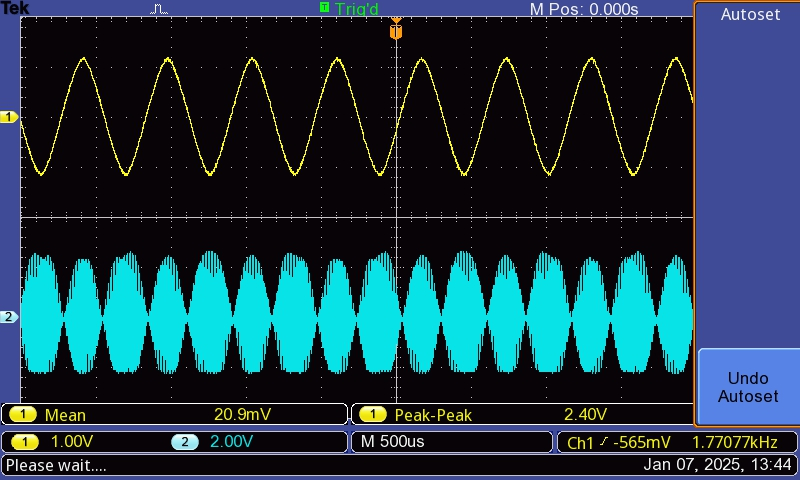
\includegraphics[width=\linewidth]{p3-msg-100mod.JPG}
        \caption{AM; Yellow: Message, Blue: 100\% Modulated}
        \label{fig:pic3}
    \end{minipage}
    \hfill
    \begin{minipage}{0.45\linewidth}
        \centering
        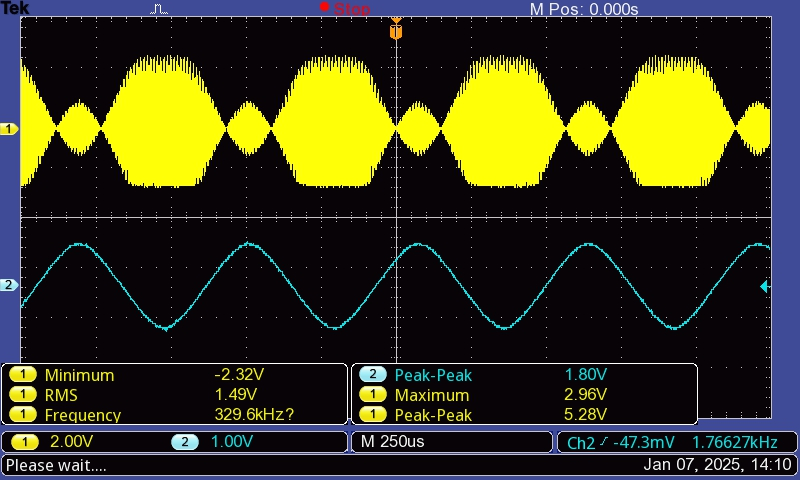
\includegraphics[width=\linewidth]{p4-ovMod-msg.JPG}
        \caption{AM; Yellow: Over-modulated, Blue: Message}
        \label{fig:pic4}
    \end{minipage}
    \vspace{1em}
    \begin{minipage}{0.45\linewidth}
        \centering
        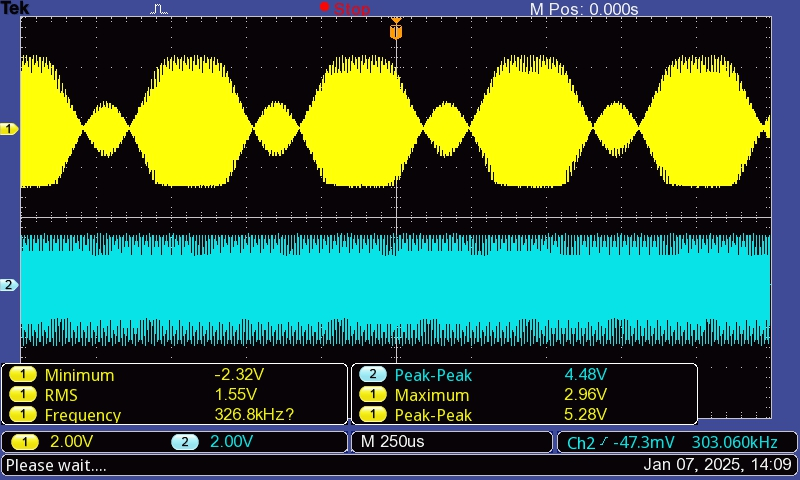
\includegraphics[width=\linewidth]{p5-ovMod-car.JPG}
        \caption{AM; Yellow: Over-modulated, Blue: Carrier}
        \label{fig:pic5}
    \end{minipage}
    \hfill
    \begin{minipage}{0.45\linewidth}
        \centering
        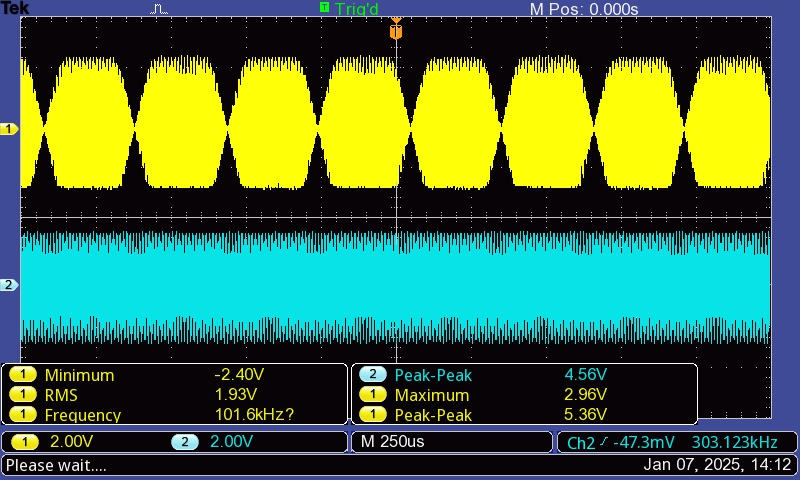
\includegraphics[width=\linewidth]{p6-dsb-mod-car.JPG}
        \caption{DSB\-SC; Yellow: Modulated, Blue: Carrier}
        \label{fig:pic6}
    \end{minipage}
\end{figure}

\pagebreak

\begin{figure}[H]
    \centering
    \begin{minipage}{0.45\linewidth}
        \centering
        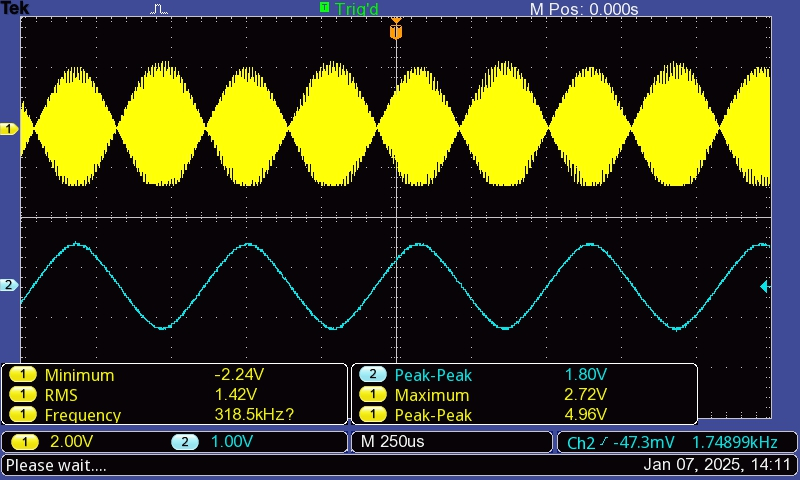
\includegraphics[width=\linewidth]{p7-dsb-mod-msg.JPG}
        \caption{DSB\-SC; Yellow: Modulated, Blue: Message 1}
        \label{fig:pic7}
    \end{minipage}
    \hfill
    \begin{minipage}{0.45\linewidth}
        \centering
        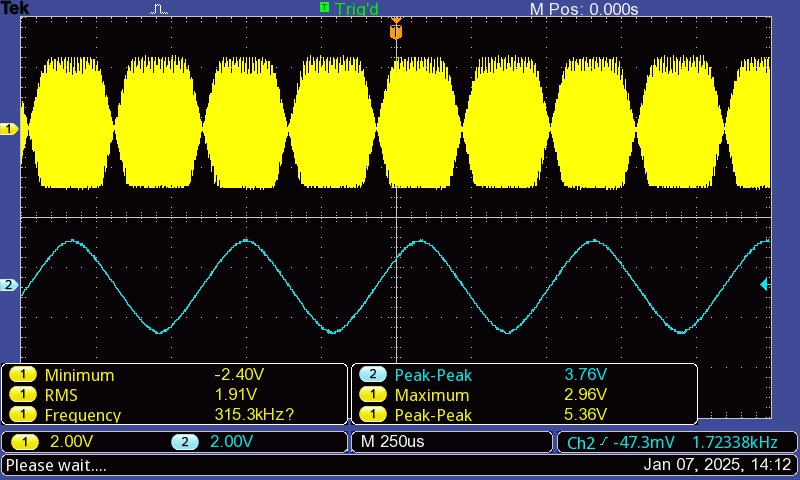
\includegraphics[width=\linewidth]{p8-dsb-mod-msg2.JPG}
        \caption{DSB\-SC; Yellow: Modulated, Blue: Message 2}
        \label{fig:pic8}
    \end{minipage}
    \vspace{1em}
    \begin{minipage}{\linewidth}
        \centering
        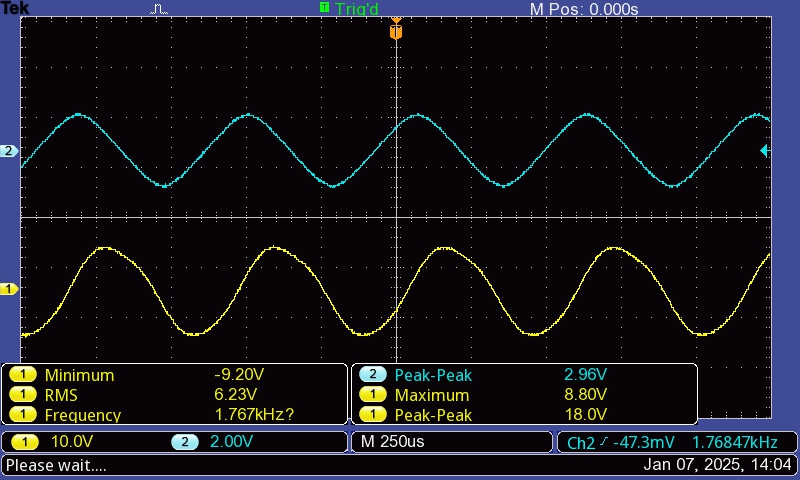
\includegraphics[width=0.4\linewidth]{p9-dsb-msg-Demod.JPG}
        \caption{DSB\-SC; Yellow: Message, Blue: Demodulated Message}
        \label{fig:pic9}
    \end{minipage}
\end{figure}

\subsection*{Matlab Simulation Output}
\addcontentsline{toc}{subsection}{Matlab Output}
\begin{figure}[H]
    \centering
    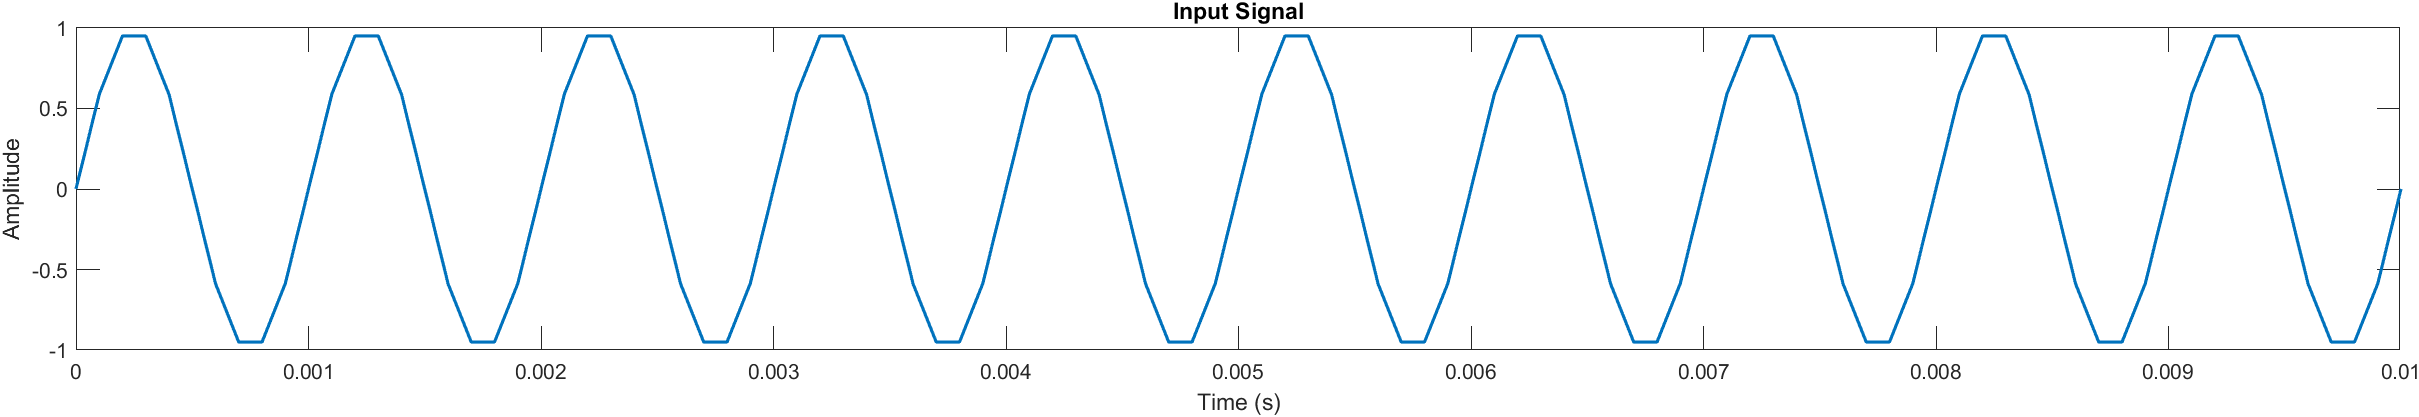
\includegraphics[width=\textwidth]{msg.png}
    \caption{Message Signal}
    \label{fig:img2}
\end{figure}

\begin{figure}[H]
    \centering
    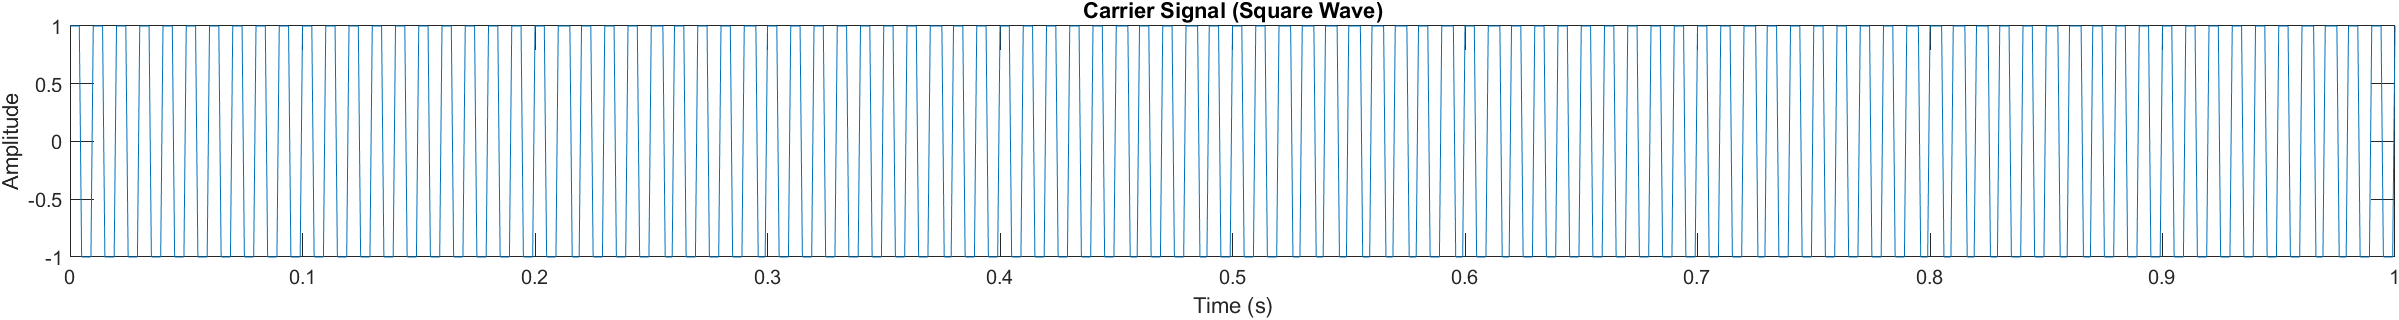
\includegraphics[width=\textwidth]{car.png}
    \caption{Carrier Signal, Square Wave}
    \label{fig:img11}
\end{figure}

\begin{figure}[H]
    \centering
    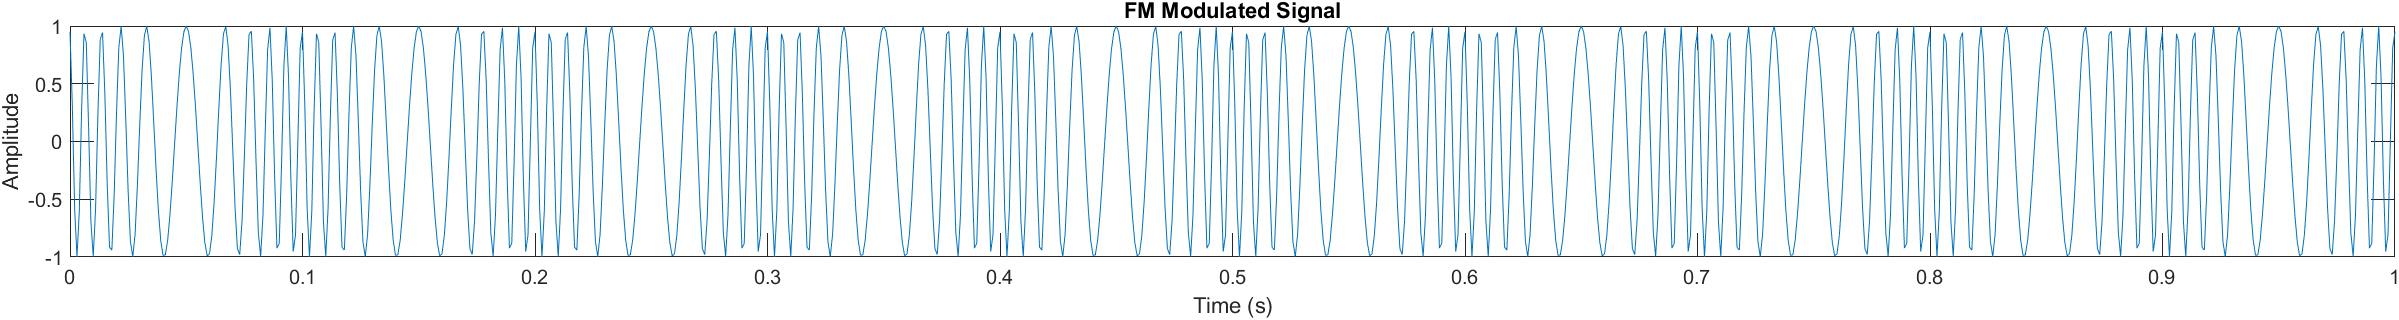
\includegraphics[width=\textwidth]{mod.png}
    \caption{FM Modulated Signal}
    \label{fig:img3}
\end{figure}

\begin{figure}[H]
    \centering
    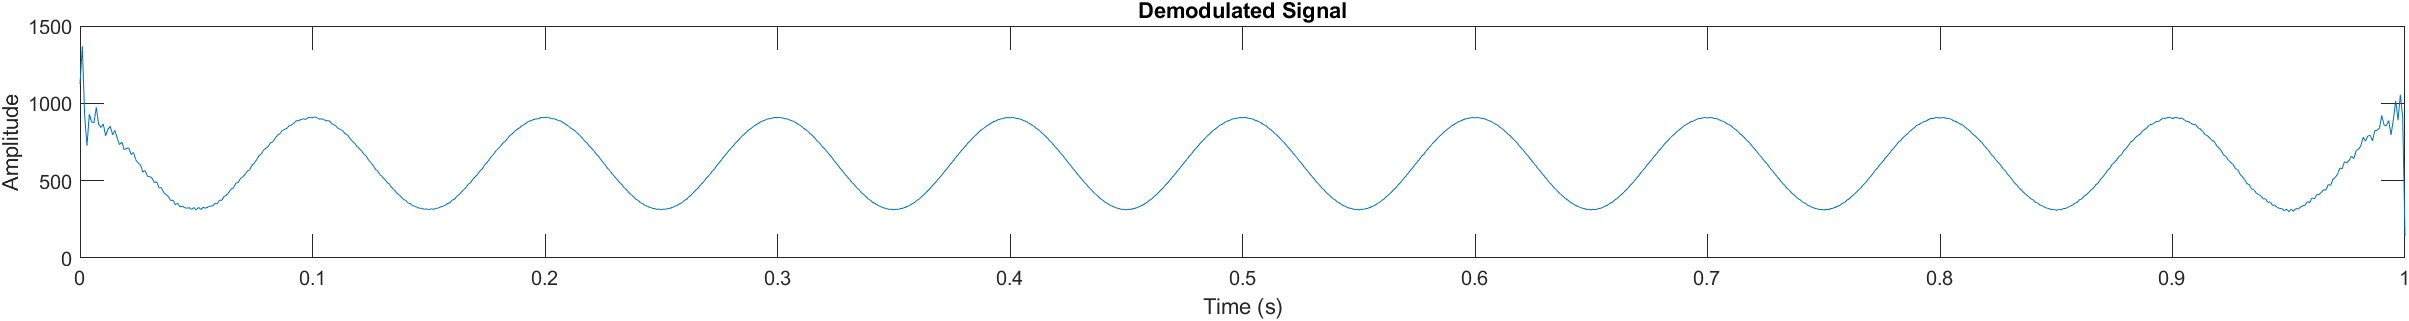
\includegraphics[width=\textwidth]{demod.png}
    \caption{Demodulated Signal}
    \label{fig:img4}
\end{figure}


\section*{Discussion and Conclusion}
\addcontentsline{toc}{section}{Discussion and Conclusion}
The experiment aimed to study digital modulation techniques: Amplitude Shift Keying (ASK), Frequency Shift Keying (FSK), and Phase Shift Keying (PSK). Using specific modulation and demodulation kits, we observed the modulated and demodulated signals on an oscilloscope and compared them with the original input signals.
\\\\
In ASK, the carrier signal's amplitude changed with the binary data, present for 1 and absent for 0. In FSK, the frequency changed, with \( f_1 \) for 1 and \( f_2 \) for 0. In PSK, the phase changed, with 0 for 1 and \( \pi \) for 0. For ASK demodulation, the demodulated signal matched the original binary data by detecting the carrier signal's presence or absence. However, a slight curve in the demodulated message signal indicated it was not a perfect digital signal.
\\\\
In conclusion, the experiment demonstrated the principles of ASK, FSK, and PSK modulation and demodulation. The oscilloscope observations confirmed the theoretical expectations. The slight imperfection in the ASK demodulated signal suggests minor distortions in real-world implementations, which should be considered in practical applications. Overall, the experiment provided valuable insights into digital modulation techniques and their practical implications.

\bibliographystyle{IEEEtran}
\renewcommand{\bibname}{References}
\addcontentsline{toc}{section}{References}
\bibliography{ref}

\end{document}
